\section{Requirements}
\label{requirement}

\subsection{Preliminary Analysis}
We first performed analysis on the given proposal in Section \ref{scope}. On the infrastruture side, the proposal requires the project to be integrated into Jira. Among the different versions of Jira software available, the team chose Jira Cloud over Jira Server, for its cloud-based nature is more compatible in modern workplace. 

We defined the key concepts as given in the primary requirements. For the purpose of our project, we consider
\textbf{Epic} to be a collection or narrative of user stories; they contain more information as to the functional usage of a target project being documented. The next level is \textbf{User Story}, which is a compact set of requirements. These requirements can be furthered broken down into \textbf{Tasks}, actionable item to be completed as part of a user story. 
We consider Epic, User Story, and Tasks as the three levels of requirements items that our tool focuses on. 

\subsection{Requirement Modeling with KAOS}
First, the team modeled the requirements through the use of KAOS models\cite{KAOS}. KAOS is a Goal-oriented requirement engineering \cite{GOAL} tool that emphasizes goals in requirement acquisition. The team built the KAOS models to build thorough traceabilities within project requirements, which includes describing the problem to be solved, identifying top level goals to address problems, the constraint it must be fulfilled by solutions, etc. Moreover, using the KAOS models, the team could easily remove or add requirements as we encounter new information and changes. \cite{KAOS} provides universally applicable patterns for reference, and we specified our initial goals by adopting these generic patterns, which also guide the later requirement refinement.

\begin{figure}
\centering
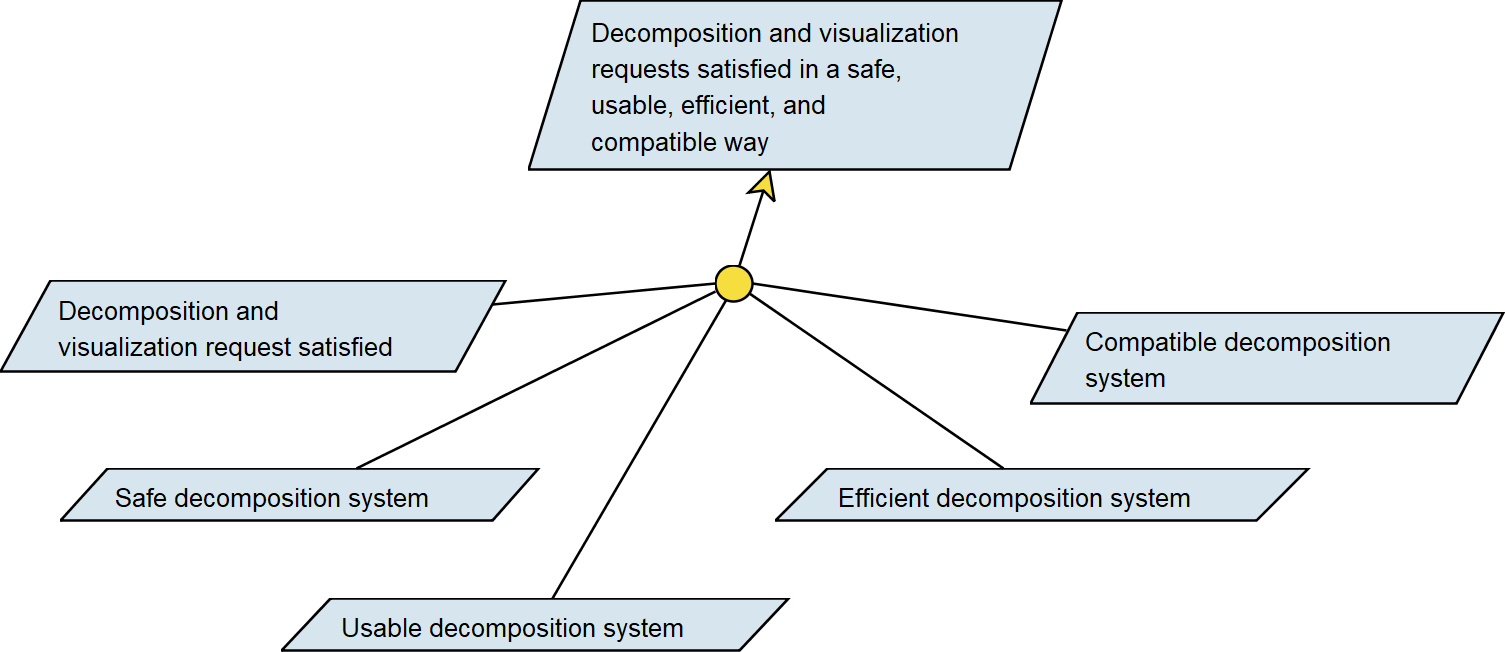
\includegraphics[width=\textwidth,keepaspectratio]{./figure/GoalsNFR1.png}
\caption{Goal: “Decomposition requests satisfied in a secure, usable, efficient, compatible, and reliable way”.}
\label{goal1}
\end{figure}

We identify three primary processes to handle the requirements items defined above: 1) Epic Decomposition, 2) Story Optimization, and 3) Task Generation. Fig. \ref{goal1} defines the top-level goal for the entire system, with subgoals that enumerate all the cases that must be covered to fulfill our main goal. The subgoals each encompasses a portion of the functional and nonfunctional requirements (FRs and NFRs) of the system. As shown in Fig. \ref{goal1}, the goals that our system should achieve are:

\begin{itemize}
	\item Decomposition and visualization request satisfied
	\item Safe decomposition system
	\item Usable decomposition system
	\item Efficient decomposition system
	\item Compatible decomposition system
\end{itemize}

The goals for “Safe System”, “Usable System”, “Efficient System”, and “Compatible System” covered the NFR portion of the system. By using respective generic patterns from \cite{KAOS}, we generated the nonfunctional requirements for our system as shown in Table \ref{nfrs}.

%\begin{center}
\begin{table}
\centering
\caption{Non-functional requirements}
\label{nfrs}
\begin{tabular}{ |c|c| } 
\hline
\multicolumn{1}{|c|}{\textbf{ID}} & \multicolumn{1}{c|}{\textbf{Description}} \\
\hline
NFR1 & Show resources about Agile development \\
\hline
NFR2 & Follow Agile development process \\
\hline
NFR3 & Have presets for user without domain expertise \\
\hline
NFR4 & Show notification about decomposition status \\
\hline
NFR5 & Do not store information on third-party database \\
\hline
NFR6 & Only query Jira the information that is needed \\
\hline
NFR7 & Software is secure \\
\hline
NFR8 & Retain original sentences in epics with minimal modification \\
\hline
NFR9 & The response time for AI processing is less than five seconds \\
\hline
NFR10 & The response time for visualization is less than two seconds \\
\hline
NFR11 & Visualization only generates important relationships \\
\hline
NFR12 & Available on Atlassian Marketplace \\
\hline
NFR13 & Available on Atlassian Partner Marketplace \\
\hline
\end{tabular}
\end{table}
%\end{center}

\begin{figure}
\centering
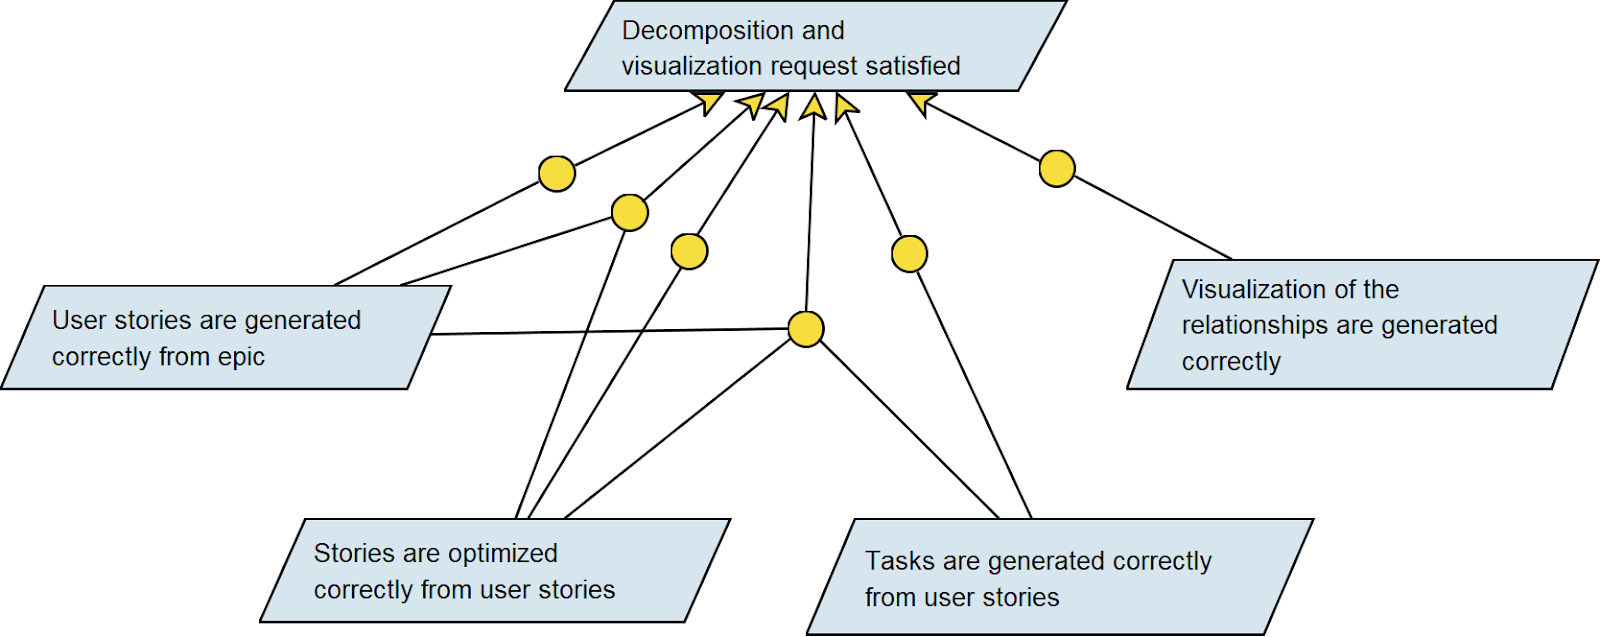
\includegraphics[width=\textwidth,keepaspectratio]{./figure/GoalsNFR2.png}
\caption{Goal: “Decomposition request and visualization satisfied”.}
\label{frgs}
\end{figure}

Next, we broke down the “decomposition request and visualizations satisfied” goal into subgoals, which correlated to the main FRs. Fig. \ref{frgs} shows the first level of functional subgoals, also listed below: 

\begin{itemize}
	\item User stories are generated correctly from epic
	\item Stories are optimized correctly from user stories
	\item Tasks are generated correctly from user stories
	\item Visualization of the relationships are generated correctly
\end{itemize}

Each subgoal in Fig. \ref{frgs} has its own KAOS goal model to be further refined. Due to space constraint, we include one example in Fig. \ref{fr1} to demonstrate the refinement from subgoal ``User stories are generated correctly from epic'' to the specification, as well as responsible agent for fulfillment.  From these models, we concluded the functional requirements as in Table \ref{frt}.

\begin{figure}
\centering
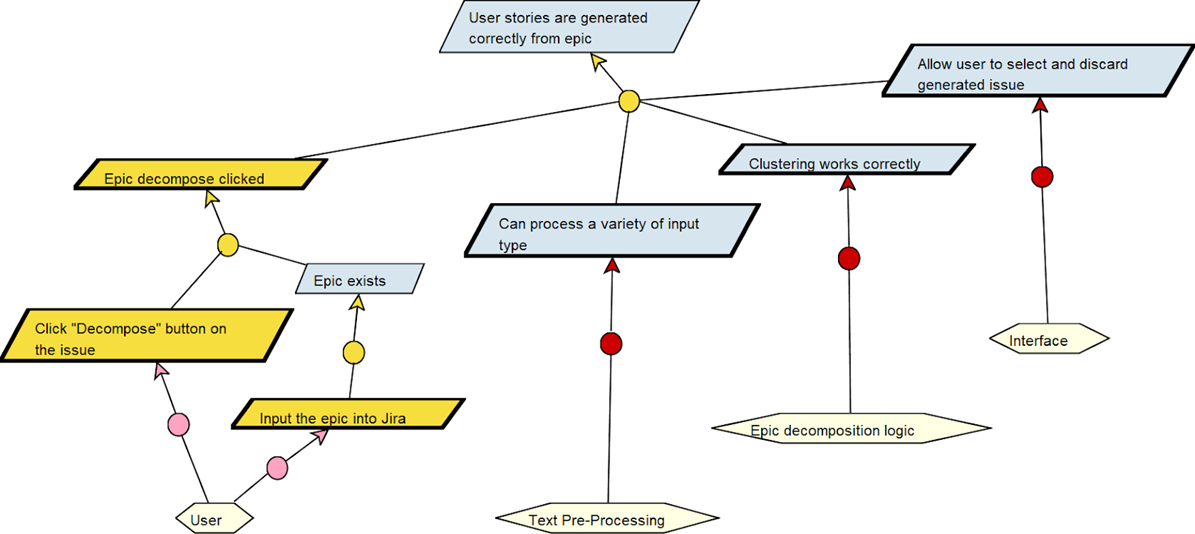
\includegraphics[width=\textwidth]{./figure/GoalsFR1.png}
\caption{Goal: “User stories are generated correctly from epic”.}
\label{fr1}
\end{figure}

\begin{table}
\centering
\caption{Functional requirements}
\label{frt}
\begin{tabular}{ |c|c| } 
\hline
\multicolumn{1}{|c|}{\textbf{ID}} & \multicolumn{1}{c|}{\textbf{Description}} \\
\hline
FR1 & Clustering works correctly \\
\hline
FR2 & Allow user to select and discard generated issue \\
\hline
FR3 & Can process a variety of input types \\
\hline
FR4 & User stories extraction works correctly \\
\hline
FR5 & Retain user stories if those are small enough \\
\hline
FR6 & Sentence building works correctly \\
\hline
FR7 & Show the explicit relationship between issues as a tree \\
\hline
FR8 & Show the implicit relationship of developers to the issues as clusters \\
\hline
FR9 & Allow user to show and edit relationship \\
\hline
FR10 & Show a customizable type and depth to relationship between issues \\
\hline
FR11 & The graph should render as the object is selected \\
\hline
\end{tabular}
\end{table}

\subsection{Requirements Summary}
The NFRs and FRs listed in Tables \ref{nfrs} and \ref{frt} are the scope of our implementation, each with their own specifications developed as well. To summarize the system's three major functional processes, we conclude that: 1) Epic decomposition consists of taking a semi-structured epic, entered by the user, and clustering requirements together into user stories based upon subject; 2) Story optimization further breaks down potentially large stories into smaller stories. Certain stories may not be subjected to change due to their intial small size; 3) Task generation is done by performing part of speech analysis on the user stories. 

Furthermore, to achieve the NFRs such as integrity, for each process, the results are offered as suggestions to the user, allowing them to pick and choose which user stories and tasks to add to their Jira board. The user can further adjust settings to fine tune the granularity of generated results. i.e. number of tasks to be generated. Last but not least, epics, user stories, and tasks may be displayed in an interactive tree/cluster graph that shows the explicit and implicit relationships among them.

Overall, we consider the project's main motivation is to reduce the time needed on manual requirement engineering. While AI can play a number of different roles to achieve this goal, the team determined that the artificial intelligence component’s purpose would be centered on processing text into increasingly refined portions to support an efficient RE process. Such an approach would increase the consistency of the outcome of the process, as the central process reduces the impact of human variables. At the meantime, we recognized that knowledge from an experienced project manager is still valuable, thus we make sure that the tool would not alter or discard the original input, avoiding unintended consequences. 

Finally, the team combined the formatted requirement with direct feedback from our mentor and developed the user stories that we later used for demo and verification purposes, as presented in Section \ref{demo}.